\section{Ejercicio 3}

\subsection{Enunciado}

Programar un tipo de tarea \textbf{TaskBatch} que reciba dos parámetros: \textit{total\_cpu} y \textit{cant\_bloqueos}. Una tarea de este tipo deberá realizar \textit{cant\_bloqueos} llamadas bloqueantes, en momentos elegidos seudoaleatoriamente. En cada tal ocasión, la tarea deberá permanecer bloqueada durante exactamente dos (2) ciclos de reloj. El tiempo de CPU total que utilice una tarea \textbf{TaskBatch} deberá ser de \textit{total\_cpu} ciclos de reloj (incluyendo el tiempo utilizado para lanzar las llamadas bloqueantes; no así el tiempo en que la tarea permanezca bloqueada). Explique la implementación realizada y grafique un lote que utilice 4 tareas \textbf{TaskBatch} con parámetros diferentes y que corra con el scheduler \textbf{FCFS}. 

\textbf{HINT}: Piense en distribuir adecuadamente esas llamadas bloqueantes. Algunos suelen llamarlo \textit{shuffle}.


\subsection{Resolución}

Para el ejercicio programamos la tarea TaskConsola de la siguiente forma:

\begin{lstlisting}
void TaskBatch(int pid, vector<int> params) {
	// params: total_cpu cant_bloqueos
	
	// Entero que utlizamos para generar el valor pseudoaleatorio
	int random_num;
	
	// Pasamos los valores de params a variables mas declarativas
	int total_cpu = params[0];
	int cant_bloqueos = params[1];
	
	// El total del cpu que se utilice va a ser total_cpu - cant_bloqueos (ya que por 
	// cada uno de ellos se utiliza 1 ciclo del cpu) y - 1 ya que return utiliza 
	// un ciclo de reloj.
	int cpu_restante = total_cpu - cant_bloqueos - 1;

	// Ciclo mientras todavia haya bloqueos para realizar
	while(cant_bloqueos > 0){
		// Genero un numero aleatorio entre 0 y cpu_restante
		random_num = rand() % (cpu_restante + 1);
		
		// Si el numero aleatorio es mayor que cero, uso el CPU
		// random_num ciclos.
		if(random_num > 0) uso_CPU(pid, random_num);
		
		// Descuento random_num ciclos a cpu_restante
		cpu_restante = cpu_restante - random_num;
		
		// Se realiza la llamada bloqueante
		uso_IO(pid, 2);
		
		cant_bloqueos--;
	}
	return;
}
\end{lstlisting}

Cómo debemos realizar \textit{cant\_bloqueos} llamadas bloqueantes, en momentos elegidos pseudoaleatoriamente, lo que hacemos con este código es utlizar el CPU con una cantidad aleatoria de ciclos (entre 0 y \textit{cpu\_restante}) y luego se realiza la llamada bloqueante. Esto genera que las llamadas bloqueantes se realicen efectivamente en momentos pseudoaleatoriamente.

La variable \textit{cpu\_restante} se genera restandole a \textit{total\_cpu} la cantidad de bloqueos más uno. Esto es porque cuando se llama a la función \textbf{uso\_IO} se utiliza un clock de CPU y el uno restante es porque la función \textbf{return} también utiliza un clock de CPU.

Generamos y ejecutamos el siguiente lote, y luego graficamos la simulación usando el algoritmo FCFS con un costo de 3 clocks para cambiar de contexto.

\begin{center}
	\begin{tabular}{|l|}
		\hline
							\\
		TaskBatch 23 1		\\
		@5: 				\\
		TaskBatch 42 2		\\
		@6:					\\
		TaskBatch 58 3		\\
		@8:					\\
		TaskBatch 77 4		\\
							\\
		TaskBatch 33 12		\\
		@2:					\\
		TaskBatch 50 5		\\
		@3:					\\
		TaskBatch 70 9		\\
		@2:					\\
		TaskBatch 27 3		\\
							\\
		\hline
	\end{tabular}
\end{center}

\begin{figure}[!h]
	\begin{center}
		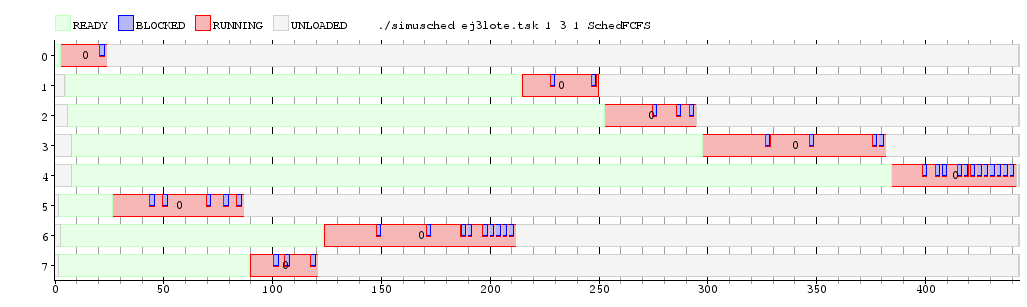
\includegraphics[width=500px]{imagenes/ej3.png}
		\caption{\small{\textbf{Gráfico generado con el lote.}}}
		\label{fig:grafico_ej1}
	\end{center}
\end{figure}